\subsection{Network Architecture and Hyperparameters}

\subsubsection{Network}
As outlined in section (\ref{subsec:model_based_optimal_control}), the policy network used by DEQNs is a Multilayer Perceptron (MLP), consisting solely of densely connected layers. The specific architecture employed in this thesis follows those of the works by \textcite{Azinovic2022DEQN, friedl2023_deepUQ, Folini2024ClimateInCE}\footnote{\textcite{Folini2024ClimateInCE} does not cover the specific architecture for their policy network in the paper. However, they have a GitHub repository accompanying the paper.}. Table (\ref{table:Network_Architecture}) lists each layer with the respective characteristics, and figure (\ref{fig:pol-net-architecture}) is an illustration of the architecture. 

\begin{table}[ht]
\centering
\begin{tabular}{llll}
    \toprule
    Layer Number & Layer Type & Nodes & Activation Function \\
    \midrule
    1 & Input Layer & \(|\mathcal{S}|=7\) & None \\
    2 & Dense & 1024 & ReLu \\
    3 & Dense & 1024 & ReLu \\
    4 & Output Layer & \(|\mathcal{A}|=11\) & Action Specific \\
    \bottomrule
\end{tabular}
\caption{Network Architecture}
\label{table:Network_Architecture}
\end{table}

The input layer takes the state vector, which in the case of the DICE variations of ACE has a state space that is given by \(\bm{s}_t \in \mathbb{R}^7\). Therefore, the size of the input layer is 7. This is followed by two hidden layers, each comprising 1024 neurons. These layers utilize the ReLU (Rectified Linear Unit) activation function. The output layer gives the action vector, which in the case of the DICE variations of ACE is \(\bm{a}_t \in \mathbb{R}^{11}\), meaning that it has 11 units. These outputs are then fed to specific activation functions that map the raw output of the MLP to the appropriate ranges.

\textcite{friedl2023_deepUQ} distinguishes itself from the other papers by using the self-normalizing Scaled Exponential Linear Unit (selu) activation function \parencite{klambauer2017selfnormalizing} in the hidden layers. However, in the interest of simplicity and computational efficiency, I followed the approach of the other two papers and used the relu activation function. The relu function has performed well in previous studies and is easier to compute.

\begin{figure}[ht]
    \centering
    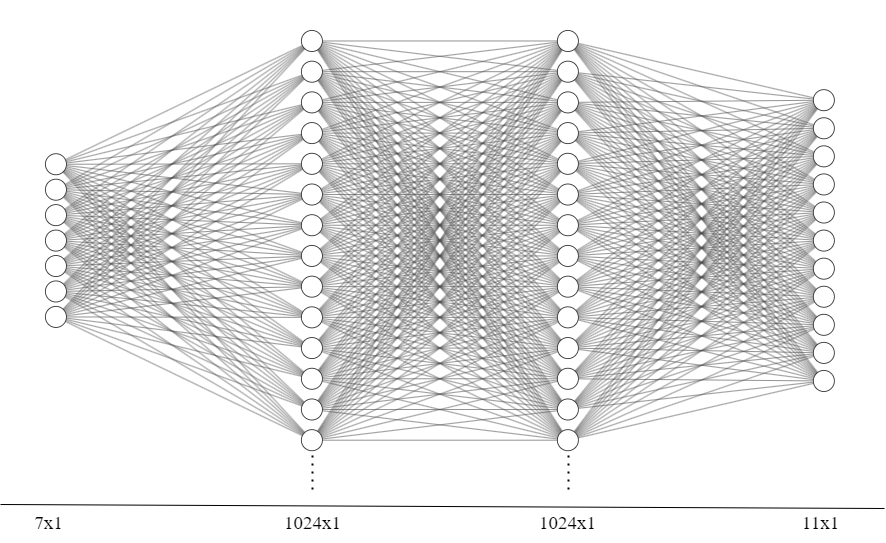
\includegraphics[width=0.9\textwidth]{images/ch6/pol-net-architecture.png}
    \caption{Illustration of policy network architecture}
    \label{fig:pol-net-architecture}
\end{figure}

The output layer has specific activation functions tailored to each action variable. The same custom activation functions were utilized in the output layer in both model runs, as detailed in Table (\ref{table:Custom_Activation_Functions}). The activation functions applied to the costate variables largely mirror those found in \textcite{Folini2024ClimateInCE}, where a linear activation function is applied to each respective costate variable. Each linear output is multiplied by a fixed scale \(c\) that matches the order of magnitude of the variable, so that the network itself only has to produce numbers of order one.

\begin{table}[ht]
\centering
\begin{tabular}{lll}
    \toprule
    Action Variable & Activation Function & Function Mappings \\
    \midrule
    \(x_t\) & Custom Sigmoid & \(f: \mathbb{R} \to (\alpha, 1-\alpha)\), \(\alpha\) small \\
    \(E_t\) & Custom Sigmoid & \(f: \mathbb{R} \to (\alpha, E_t^\text{BAU}(1-\alpha))\), \(\alpha\) small \\ 
    \(V_t\) & Scaled linear, \(c_V = 30\) & \(f: \mathbb{R} \to (-\infty, \infty)\) \\ 
    \(\lambda_{k,t}\) & Linear, \(c_k = 1\) & \(f: \mathbb{R} \to (-\infty, \infty)\) \\
    \(\bm{\lambda}_{M,t}\) & Scaled linear, \(c_M = 10^{-4}\) & \(f: \mathbb{R} \to (-\infty, \infty)\) \\
    \(\bm{\lambda}_{\tau,t}\) & Scaled linear, \(c_\tau = 10^{-1}\) & \(f: \mathbb{R} \to (-\infty, \infty)\) \\
    \(\lambda_{E,t}, \lambda_t^{\text{BAU}}\) & Scaled linear, \(c_{\text{KKT}} = 10^{-4}\) & \(f: \mathbb{R} \to (-\infty, \infty)\) \\
    \bottomrule
\end{tabular}
\caption{Custom Functions}
\label{table:Custom_Activation_Functions}
\end{table}

To prevent potential issues such as taking the logarithm of zero or dividing by zero, modifications were necessary for the activation functions of the control variables \(x_t\) and \(E_t\)\footnote{Refer to appendix (\ref{appendix:deqn_model_specific_mapping}) for the specific functional forms of the two model versions of ACE.}. The custom sigmoid functions scale inputs between a minimal constant \(\alpha\) and an adjusted upper limit \(b\), as depicted in the following equation:

\begin{equation}
    f(x) = b \left( \alpha + (1-2\alpha)\text{sigmoid}(x) \right)
\end{equation}

The custom sigmoid function on \(x_t\) uses \(b=1\) and the custom sigmoid function on \(E_t\) uses \(b=E_t^\text{BAU}\) in both versions, while land-use emissions \(E_t^\text{land}\) enter the carbon cycle exogenously. The bounded emissions are computed once from the raw network output, and the same value is used in the equations of motion and in every objective function.

\subsubsection{Scaling of the Objective Functions}
\label{subsubsec:objective_scaling}

The costate variables differ by several orders of magnitude. At the analytical solution, \(\lambda_{k} \approx 0.35\), while \(\lambda_{M_1} \approx -10^{-4}\). The residuals of the conditions involving the carbon costates are correspondingly small, so in an unweighted sum of squares the carbon conditions \(\ell_1\) and the emissions condition \(\ell_4\) would barely affect the policy objective, and the network could leave the SCC almost undetermined. I therefore divide each residual by the scale of the costate it pins down: \(\ell_1\) and \(\ell_4\) by \(c_M\), and \(\ell_2\) by \(c_\tau\). The Fischer-Burmeister functions are evaluated on the scale-free pairs \((\lambda_{E,t}/c_{\text{KKT}},\, E_t/E_t^\text{BAU})\) and \((\lambda^\text{BAU}_t/c_{\text{KKT}},\, 1 - E_t/E_t^\text{BAU})\). Dividing a residual by a positive constant changes neither its root nor the solution of the system, only how strongly each condition is weighted in the policy objective (eq. \ref{eq:total_objective_function}).


\subsubsection{Training Scheme}

\textcite{friedl2023_deepUQ} implemented a training scheme characterized by a gradual increase in episode length as the policy network stabilized in learning. It started with an episode length of 4 and increased in powers of two, where they, in the final step, went to 300 steps. Furthermore, they used a learning rate of 1e-5 throughout the whole training process. Minibatches were adjusted from 64 to 128 as the network became more stable.

In contrast, the publication by \textcite{Folini2024ClimateInCE} does not provide explicit details on their training methods. However, analysis of their code indicates a similar learning rate of 1e-5, complemented by gradient clipping at a maximum value of 1.0—a technique not mentioned in \textcite{friedl2023_deepUQ}. Their approach also involves increasing episode lengths but not starting as low as in the former study, with lengths set at 50, 100, and 500 steps. Additionally, the initial training cycles consist of 1,000 iterations, escalating to a final cycle of 10,000 iterations.

\begin{table}[ht]
\centering
\begin{adjustbox}{width=\textwidth,center}
{
\begin{tabular}{lcccccc}
    \toprule
    Trajectory Length & Mini Batch Size & Epochs & Learning Rate & Gradient Clipping & Training Iterations \\
    \midrule
    128 & 32 & 4 & 1e-3 \(\to\) 1e-5 (cosine) & 1.0 (norm) & 3000 \\
    \bottomrule
\end{tabular}
} \end{adjustbox}
\caption{Training Scheme}
\label{table:Training_Scheme_Results}
\end{table}

Table (\ref{table:Training_Scheme_Results}) outlines the training scheme used for the policy network. Both versions of ACE are trained in a single cycle of 3000 iterations. Each iteration simulates one episode of 128 periods (640 years) with the current policy, shuffles the visited states, and performs four epochs of mini-batch gradient descent with mini-batches of 32 states. The Adam optimizer \parencite{kingma2017adam} starts with a learning rate of 1e-3 that decays along a cosine schedule to 1e-5, and the global norm of the gradient is clipped at 1.0. After every iteration, the policy objective is evaluated on the full episode, and the weights with the lowest value are kept for the results. On a four-core CPU, one training run takes about 20 minutes.
